\documentclass[12pt]{article}

% ============================================================
%  Template SBC (Sociedade Brasileira de Computacao)
%  Use no Overleaf: "SBC Conference Template" (fornece sbc-template.sty)
%  ou coloque o arquivo sbc-template.sty na mesma pasta deste main.tex.
%  Enunciado: ate 8 paginas, SEM abstract/resumo.
% ============================================================

\usepackage{sbc-template}
\usepackage{graphicx,url}
\usepackage[utf8]{inputenc}
\usepackage[brazil]{babel}
\usepackage{booktabs}
\usepackage{multirow}
\usepackage{float}

\sloppy

\title{Classificação de Personagens da Série \textit{The Simpsons} com
\textit{Deep Features} e Fusão Estática de Classificadores}

\author{Kaike Carvalho\inst{1}, Victor Henrique Gasparoto de Almeida\inst{1}}

\address{Departamento de Computação (DACOM) -- Universidade Tecnológica
Federal do Paraná (UTFPR)\\
Campus Campo Mourão -- Campo Mourão -- PR -- Brasil
\email{kaikecarvalho@alunos.utfpr.edu.br,
victoralmeida.2004@alunos.utfpr.edu.br}
}

\begin{document}

\maketitle

% ============================================================
\section{Introdução}
% ============================================================

Reconhecer personagens em imagens é um problema clássico de visão
computacional: combina a extração de características visuais com a classificação
supervisionada. Aqui o alvo são cinco personagens da família principal de
\textit{The Simpsons} (Bart, Homer, Lisa, Maggie e Marge), classificados a partir
de imagens estáticas. O caso não é trivial. As classes compartilham a mesma
paleta de cores e traços muito próximos, como a pele amarela e os contornos
simples, e o número de imagens por personagem é desigual. Isso deixa o
desempenho preso a dois fatores: a qualidade do descritor de características e a
robustez do classificador.

O \textit{pipeline} proposto tem três etapas. Primeiro, extrai
\textit{deep features} de um \textit{Vision Transformer} pré-treinado
(ViT-large). Em seguida, treina e avalia um conjunto de 20 classificadores de
cinco famílias: k-NN, Árvore de Decisão, SVM, \textit{Random Forest} e MLP. Por
fim, combina esses classificadores por fusão estática (\textit{voting},
\textit{weighted voting}, \textit{Top-K ensemble} e \textit{stacking}), buscando
superar o melhor modelo isolado. A avaliação segue dois protocolos: validação
cruzada de 10 \textit{folds} no conjunto de treino e um teste \textit{holdout}
no conjunto de validação que acompanha a base. São reportadas acurácia,
\textit{F1-score} macro e matrizes de confusão, além da análise do efeito da
fusão e dos pontos fortes e fracos do sistema.

% ============================================================
\section{Materiais e Métodos}
% ============================================================

\subsection{Base de Dados}

A base \textit{Simpsons} traz imagens em formato BMP separadas em cinco classes,
uma por personagem. Mantivemos a divisão que já vem nos arquivos: 226 imagens
para treino e 95 para validação (\textit{holdout}). A Tabela~\ref{tab:base}
mostra quantas imagens cada classe tem no treino. A distribuição é bem desigual:
Bart é a classe com mais exemplos, e Maggie e Marge as com menos.

\begin{table}[H]
\centering
\caption{Distribuição de imagens por classe no conjunto de treino.}
\label{tab:base}
\begin{tabular}{lccccc}
\toprule
Classe & Bart & Homer & Lisa & Maggie & Marge \\
\midrule
\textit{Imagens (treino)} & 78 & 61 & 33 & 30 & 24 \\
\bottomrule
\end{tabular}
\end{table}

\subsection{Extração de Características (\textit{Deep Features})}

Em vez de descritores manuais de cor, textura ou forma, usamos
\textit{deep features}: vetores de representação extraídos de uma rede neural
profunda já treinada, que servem de entrada para os classificadores clássicos. O
modelo escolhido foi o \textit{Vision Transformer}
\texttt{google/vit-large-patch16-224-in21k}, pré-treinado no ImageNet-21k.

O fluxo por imagem é direto. Ela é redimensionada e normalizada segundo o
pré-processamento do modelo; da saída \texttt{last\_hidden\_state} do ViT
tira-se a média ao longo dos \textit{tokens} (\textit{mean pooling}), o que
produz um vetor de 1024 características. Esse vetor passa por uma padronização
\textit{z-score} (\texttt{StandardScaler}) cujas estatísticas vêm só do conjunto
de treino, para não vazar informação da validação. A ideia por trás do ViT-large
é aproveitar a atenção para capturar relações globais na imagem, o que costuma
render boas representações mesmo quando há poucos exemplos por classe.

\subsection{Classificadores}

Montamos um \textit{pool} de 20 classificadores que cobre as cinco famílias
vistas na disciplina, cada uma com variações nos hiperparâmetros mais
importantes (Tabela~\ref{tab:clf}). Todos foram implementados em
\textit{scikit-learn}.

\begin{table}[H]
\centering
\caption{\textit{Pool} de 20 classificadores e seus hiperparâmetros.}
\label{tab:clf}
\begin{tabular}{lp{8.5cm}}
\toprule
Família & Variações \\
\midrule
k-NN & $k \in \{1,3,5,7\}$ \\
Árvore de Decisão & profundidade $\in \{5,10,15\}$; critério \textit{entropy} \\
SVM & RBF com $C \in \{0{,}1;\,1{,}0;\,10{,}0\}$; \textit{kernel} linear \\
\textit{Random Forest} & $\{10,50,100,200\}$ árvores \\
MLP & topologias $(50)$, $(100)$, $(50,25)$, $(100,50)$ \\
\bottomrule
\end{tabular}
\end{table}

\subsection{Fusão Estática de Classificadores}

Para aproveitar a complementaridade entre os modelos, testamos cinco formas de
combiná-los de maneira estática sobre o \textit{pool} de 20 classificadores:

\begin{itemize}
  \item \textbf{Hard Voting}: voto majoritário entre as predições de classe.
  \item \textbf{Soft Voting}: média das probabilidades \textit{a posteriori}.
  \item \textbf{Weighted Soft Voting}: \textit{soft voting} ponderado pela
        acurácia individual de cada classificador (modelos melhores pesam mais).
  \item \textbf{Top-K Ensemble}: \textit{soft voting} apenas com os $K$ melhores
        classificadores ($K \in \{5,8,10,12,15\}$), descartando modelos fracos.
  \item \textbf{Stacking}: meta-aprendizado em que uma Regressão Logística
        (nível 1) é treinada sobre as predições dos 20 classificadores (nível 0),
        com \textit{passthrough} das características originais.
\end{itemize}

\subsection{Protocolo de Avaliação e Métricas}

A avaliação usa dois protocolos. No primeiro (A), fazemos validação cruzada
estratificada de 10 \textit{folds} sobre o treino. No segundo (B), treinamos no
conjunto de treino inteiro e medimos o desempenho no conjunto de validação
(\textit{holdout}). Relatamos três métricas: acurácia, \textit{F1-score} macro
(média por classe sem ponderação, que é a mais adequada quando a base é
desbalanceada) e a matriz de confusão $N\times N$ ($N=5$), com percentual de
acertos e erros por classe.

% ============================================================
\section{Resultados e Discussão}
% ============================================================

\subsection{Classificadores Individuais (Protocolo A: 10-fold CV)}

A Tabela~\ref{tab:ind} traz o desempenho dos 20 classificadores na validação
cruzada de 10 \textit{folds}. O mesmo resultado aparece de forma visual na
Figura~\ref{fig:acc} (acurácia individual junto dos \textit{baselines} de fusão)
e, resumido por família, na Figura~\ref{fig:fam}.

\begin{table}[H]
\centering
\caption{Acurácia e \textit{F1-score} macro dos classificadores individuais
(10-fold CV). Em destaque, os três melhores.}
\label{tab:ind}
\begin{tabular}{lcc}
\toprule
Classificador & Acurácia (\%) & F1-macro (\%) \\
\midrule
\textbf{MLP (50)}      & \textbf{88,05} & \textbf{86,85} \\
\textbf{SVM-Linear}    & \textbf{87,61} & \textbf{87,45} \\
\textbf{MLP (100,50)}  & \textbf{87,61} & \textbf{86,48} \\
MLP (100)              & 85,84 & 85,90 \\
SVM-RBF (C=10,0)       & 84,51 & 83,44 \\
MLP (50,25)            & 82,74 & 82,99 \\
SVM-RBF (C=1,0)        & 81,86 & 81,63 \\
kNN (k=3)              & 81,86 & 80,51 \\
RF (200 árvores)       & 79,65 & 76,69 \\
kNN (k=5)              & 79,20 & 75,14 \\
RF (100 árvores)       & 78,76 & 75,34 \\
kNN (k=1)              & 77,88 & 77,11 \\
kNN (k=7)              & 77,88 & 74,81 \\
RF (50 árvores)        & 74,78 & 69,19 \\
RF (10 árvores)        & 66,37 & 60,10 \\
DT (prof=10)           & 49,12 & 45,01 \\
DT (entropy)           & 49,12 & 43,48 \\
DT (prof=15)           & 49,12 & 45,01 \\
DT (prof=5)            & 46,90 & 42,20 \\
SVM-RBF (C=0,1)        & 34,51 & 10,26 \\
\bottomrule
\end{tabular}
\end{table}

O topo do ranking é ocupado pelas famílias MLP e SVM. O melhor modelo isolado,
uma MLP com camada de 50 neurônios, chega a 88,05\% de acurácia. No outro
extremo estão as Árvores de Decisão, que ficam perto de 49\% por não lidarem bem
com a alta dimensionalidade das \textit{deep features}, e o SVM-RBF com
$C=0{,}1$, que praticamente colapsa (34,51\%) por causa da regularização
excessiva. Essa distância entre o melhor e o pior modelo mostra o quanto os
hiperparâmetros importam, e é também o motivo de recorrer à fusão: ela pode somar
a força dos melhores, mas paga o preço quando os fracos entram na conta.

\begin{figure}[H]
\centering
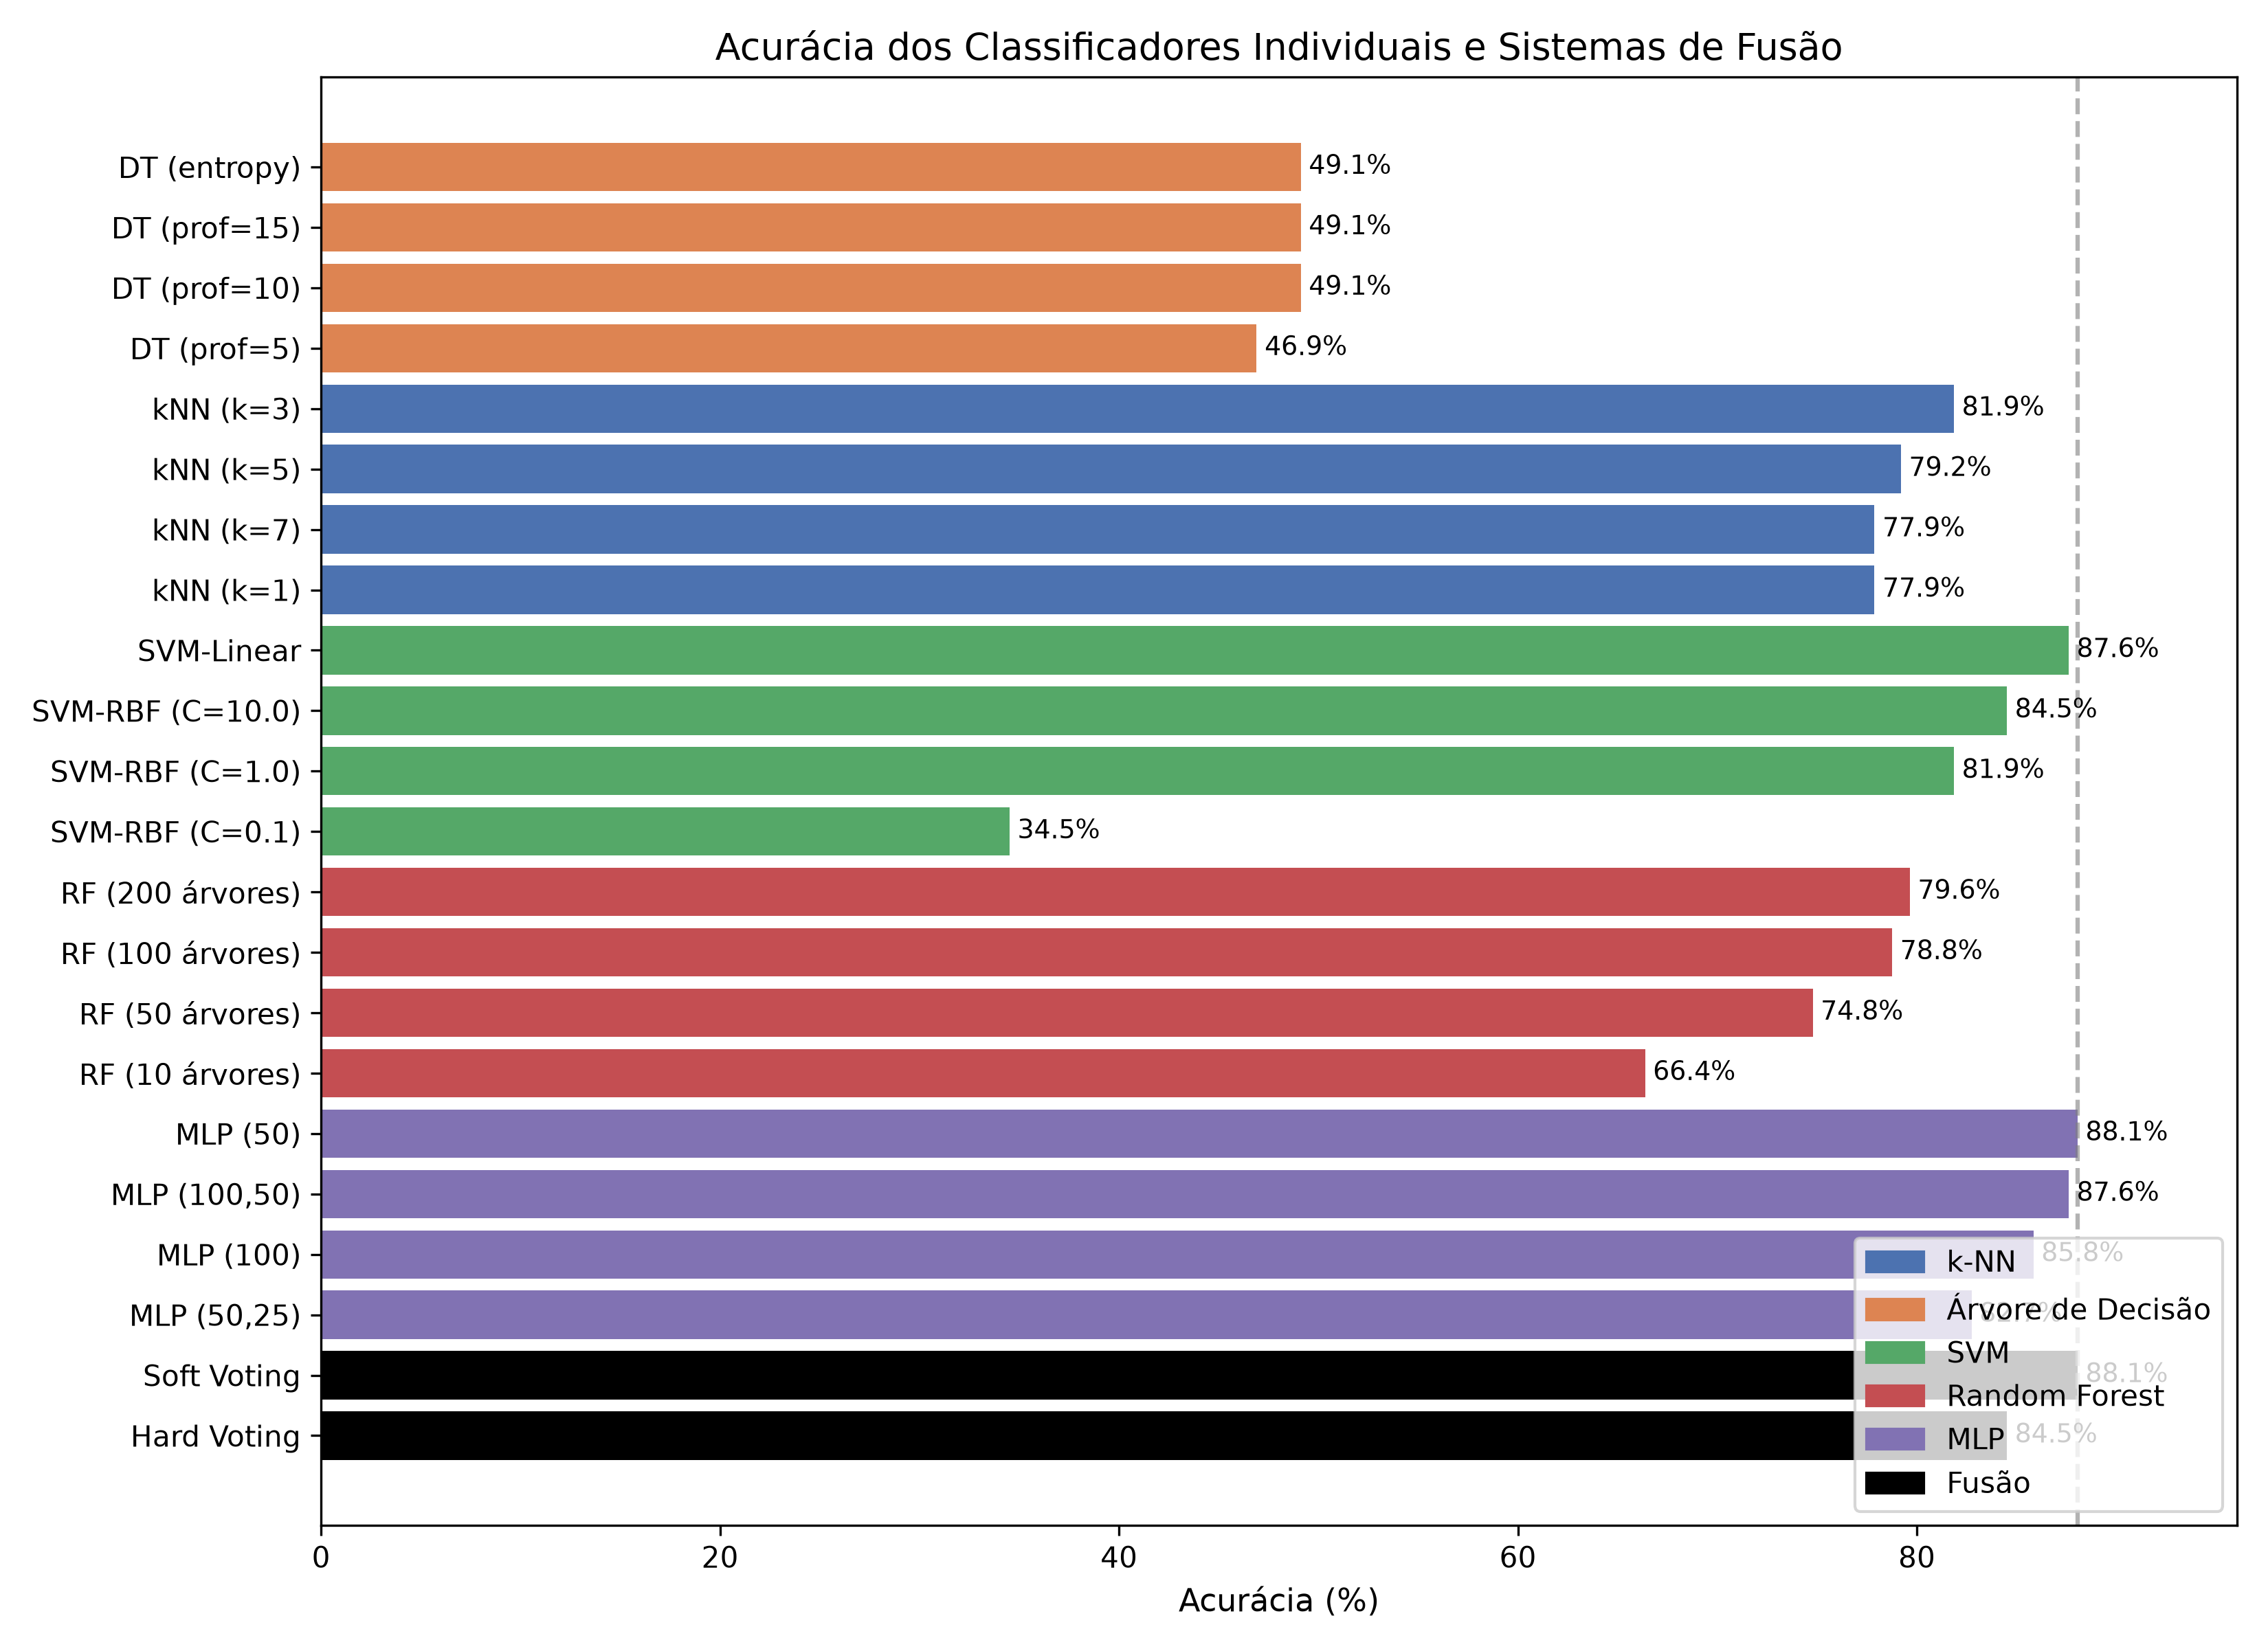
\includegraphics[width=0.78\textwidth]{figs/fig1_comparativo_acuracia.png}
\caption{Acurácia dos 20 classificadores individuais e dos \textit{baselines} de
fusão (10-fold CV), coloridos por família.}
\label{fig:acc}
\end{figure}

\begin{figure}[H]
\centering
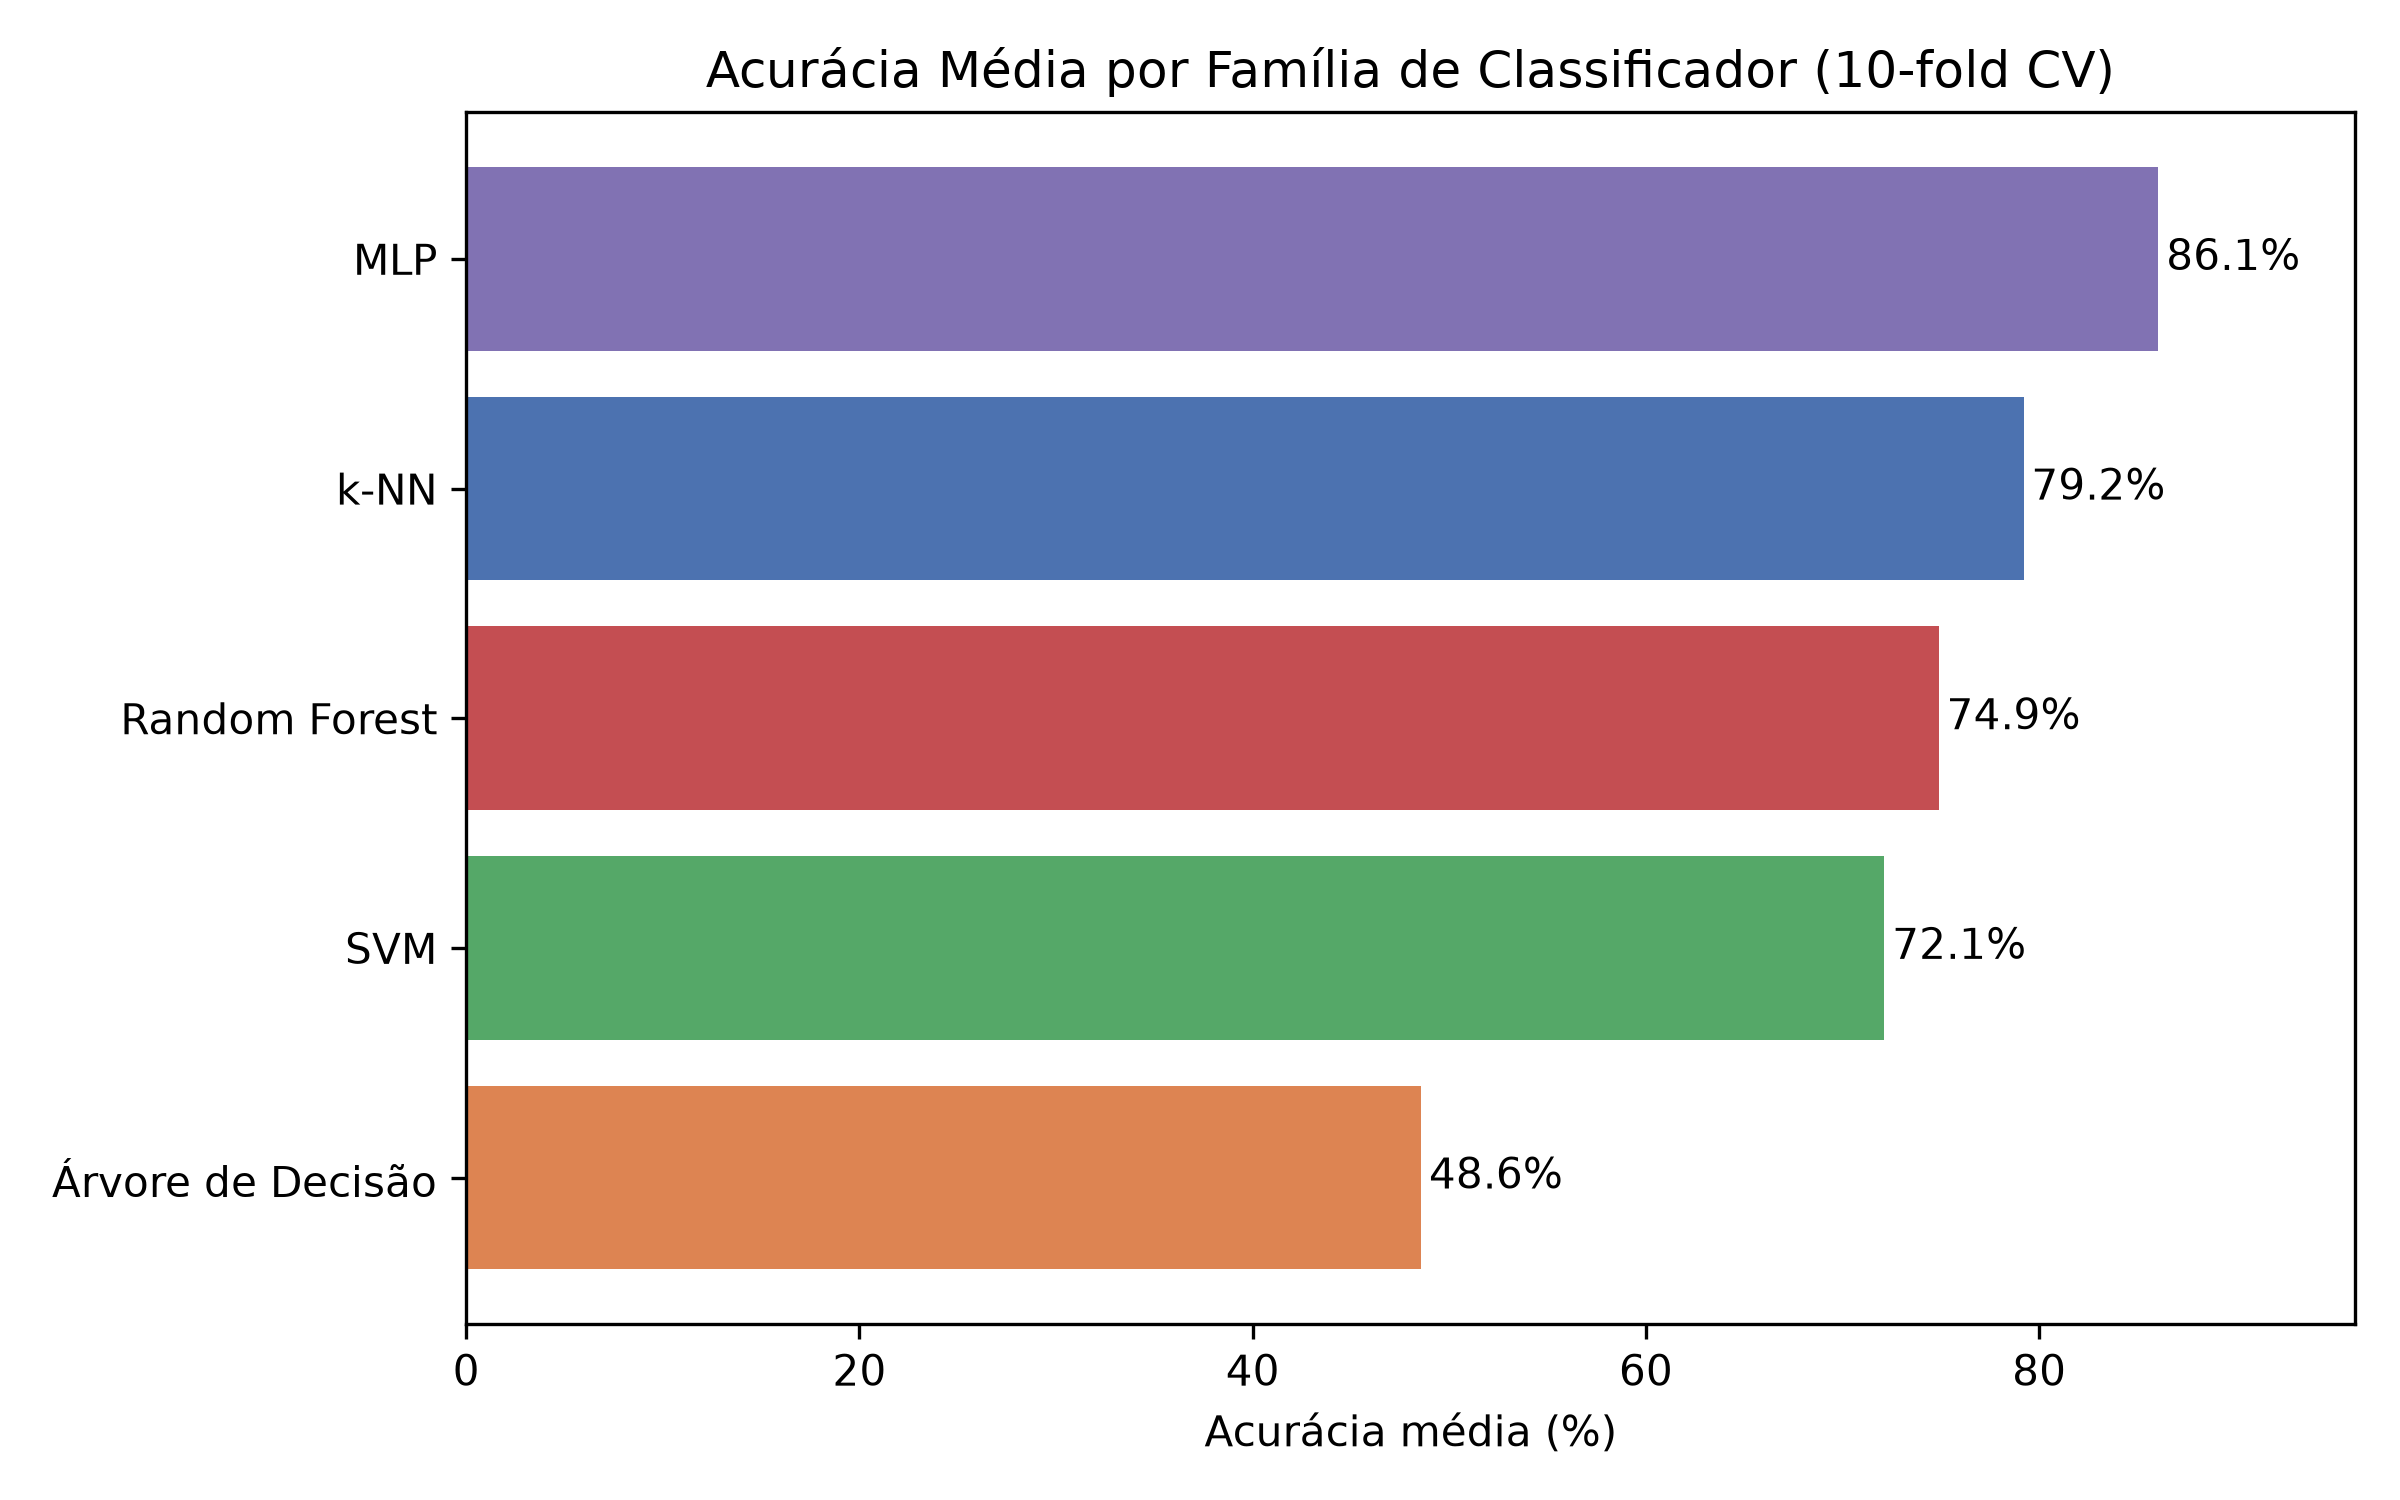
\includegraphics[width=0.56\textwidth]{figs/fig6_media_por_familia.png}
\caption{Acurácia média por família de classificador (10-fold CV).}
\label{fig:fam}
\end{figure}

\subsection{Fusão de Classificadores (Protocolo A: 10-fold CV)}

A Tabela~\ref{tab:fusao} e a Figura~\ref{fig:fusao} comparam os métodos de fusão
com o melhor classificador individual. O vencedor foi o Top-12 Ensemble, com
89,38\% de acurácia e 89,18\% de F1-macro, 1,33 ponto percentual acima da MLP 50.
O \textit{Stacking} ficou logo atrás, em 88,94\%. Já o \textit{Soft Voting} com
os 20 classificadores parou em 88,05\%, ou seja, apenas empatou com o melhor
individual, e a razão é clara: ele carrega junto os modelos fracos (as Árvores de
Decisão e o SVM-RBF $C=0{,}1$), que puxam a média para baixo.

\begin{table}[H]
\centering
\caption{Desempenho dos métodos de fusão (10-fold CV). $\Delta$ em relação ao
melhor individual (MLP 50, 88,05\%).}
\label{tab:fusao}
\begin{tabular}{lccc}
\toprule
Método & Acurácia (\%) & F1-macro (\%) & $\Delta$ (p.p.) \\
\midrule
Melhor individual (MLP 50)      & 88,05 & 86,85 & --- \\
\midrule
Hard Voting (20 clf)            & 84,51 & 83,53 & $-3{,}54$ \\
Soft Voting (20 clf)            & 88,05 & 87,84 & $+0{,}00$ \\
Weighted Soft Voting (20 clf)   & 87,61 & 87,57 & $-0{,}44$ \\
\textbf{Top-12 Ensemble (Soft)} & \textbf{89,38} & \textbf{89,18} & $\mathbf{+1{,}33}$ \\
Stacking (LR meta-learner)      & 88,94 & 88,89 & $+0{,}89$ \\
\bottomrule
\end{tabular}
\end{table}

\begin{figure}[H]
\centering
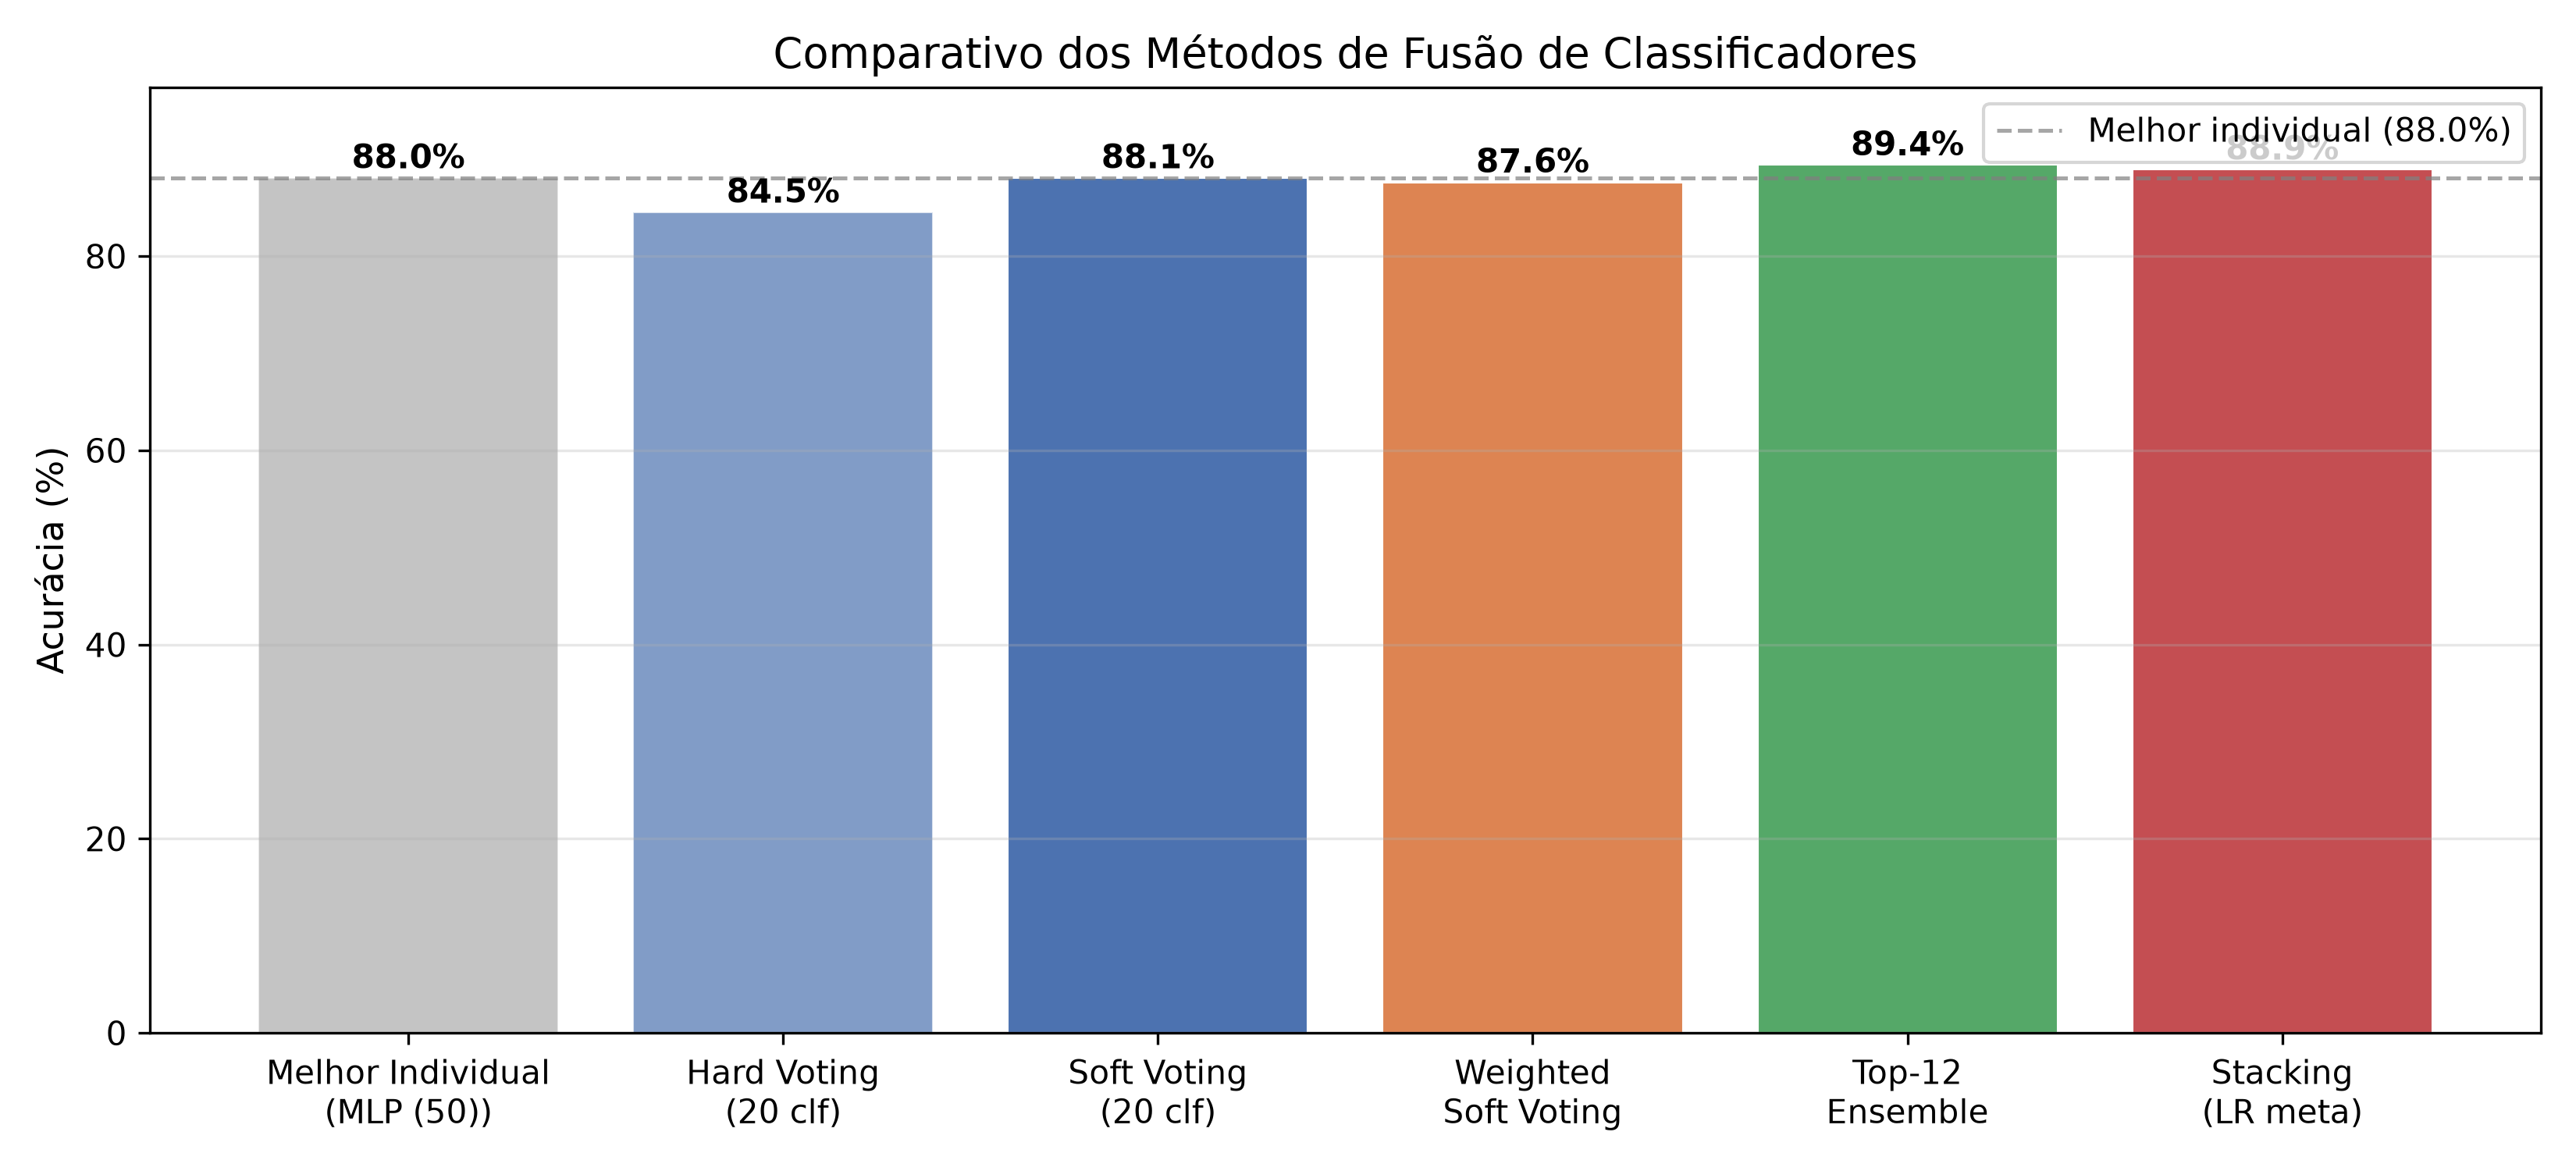
\includegraphics[width=0.80\textwidth]{figs/fig7_comparativo_fusao.png}
\caption{Comparativo dos métodos de fusão \textit{vs.} melhor individual
(10-fold CV).}
\label{fig:fusao}
\end{figure}

\textbf{Impacto da fusão.} A fusão \textit{seletiva}, de Top-K e Stacking, bate
tanto o melhor individual quanto a fusão ingênua que junta todos os modelos. Na
Figura~\ref{fig:topk} dá para ver esse efeito: a acurácia do Top-K sobe conforme
os classificadores fracos vão sendo cortados, chega ao ponto máximo em $K=12$ e
recua um pouco quando modelos piores voltam a entrar. O oposto acontece com o
\textit{Hard Voting}, o pior de todos (84,51\%): como o voto majoritário não leva
em conta a confiança de cada predição, ele acaba dominado pela massa de modelos
medianos.

\begin{figure}[H]
\centering
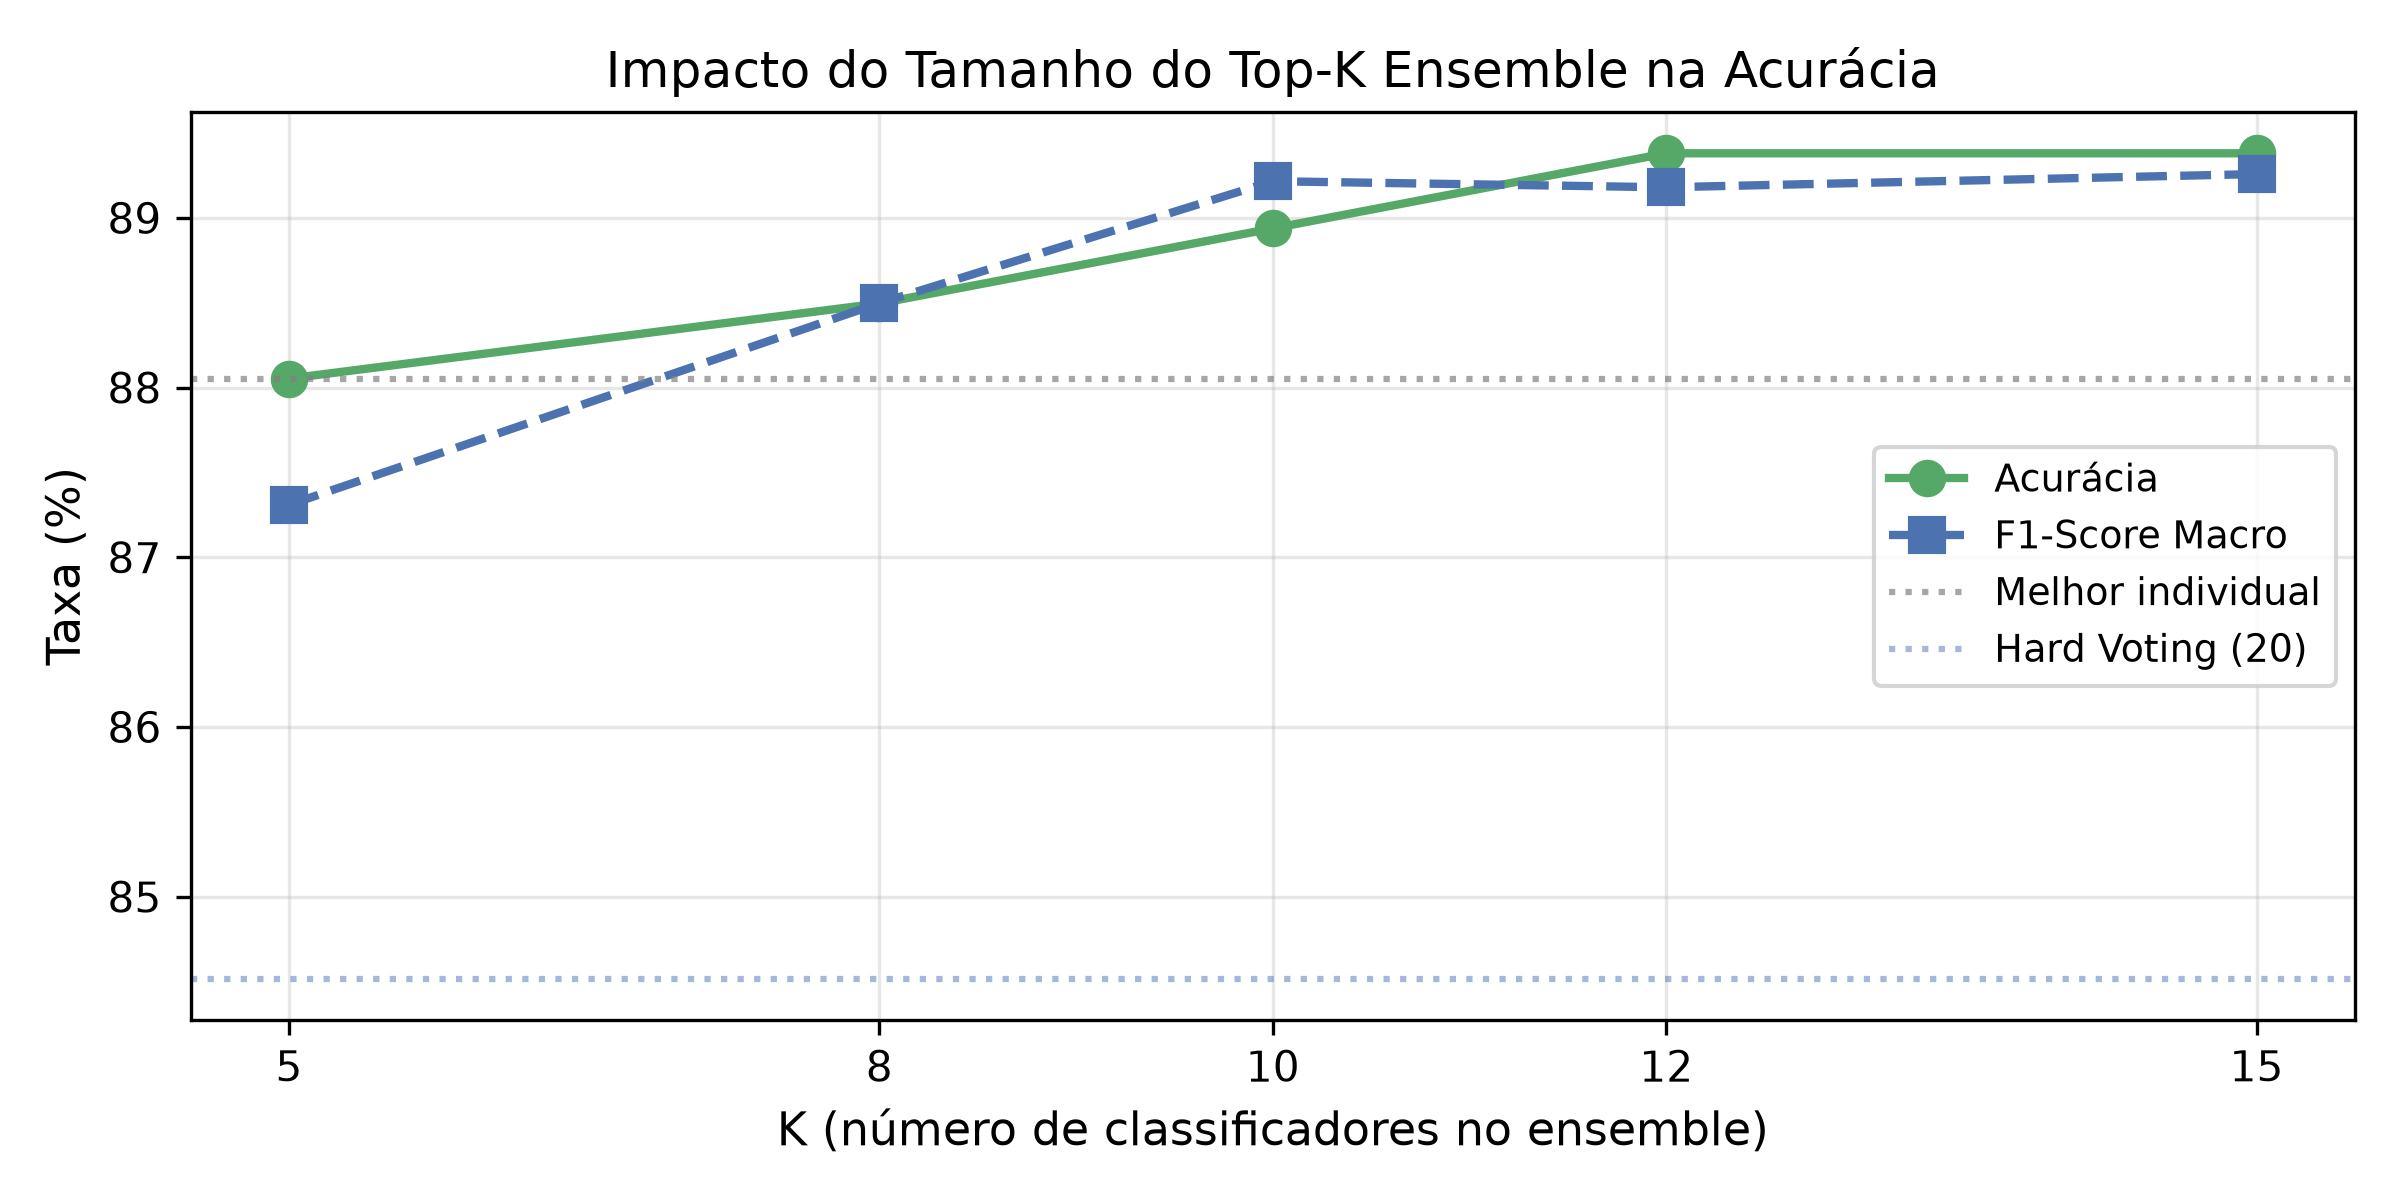
\includegraphics[width=0.62\textwidth]{figs/fig8_topk_ensemble.png}
\caption{Impacto do tamanho $K$ no \textit{Top-K Ensemble}.}
\label{fig:topk}
\end{figure}

\subsection{Matrizes de Confusão}

A Figura~\ref{fig:cm-cv} coloca lado a lado as matrizes de confusão (em \%) do
melhor classificador individual e da melhor fusão (Top-12) na validação cruzada.
Olhando classe a classe, quase todo o erro se concentra entre Maggie e Marge, as
duas personagens com menos exemplos de treino. Bart e Homer, que têm mais
imagens e são visualmente mais distintos, quase não são confundidos. A fusão
Top-12 corrige parte dessas trocas e deixa o desempenho mais parelho entre as
classes, o que se reflete no F1-macro.

\begin{figure}[H]
\centering
\begin{minipage}{0.49\textwidth}
  \centering
  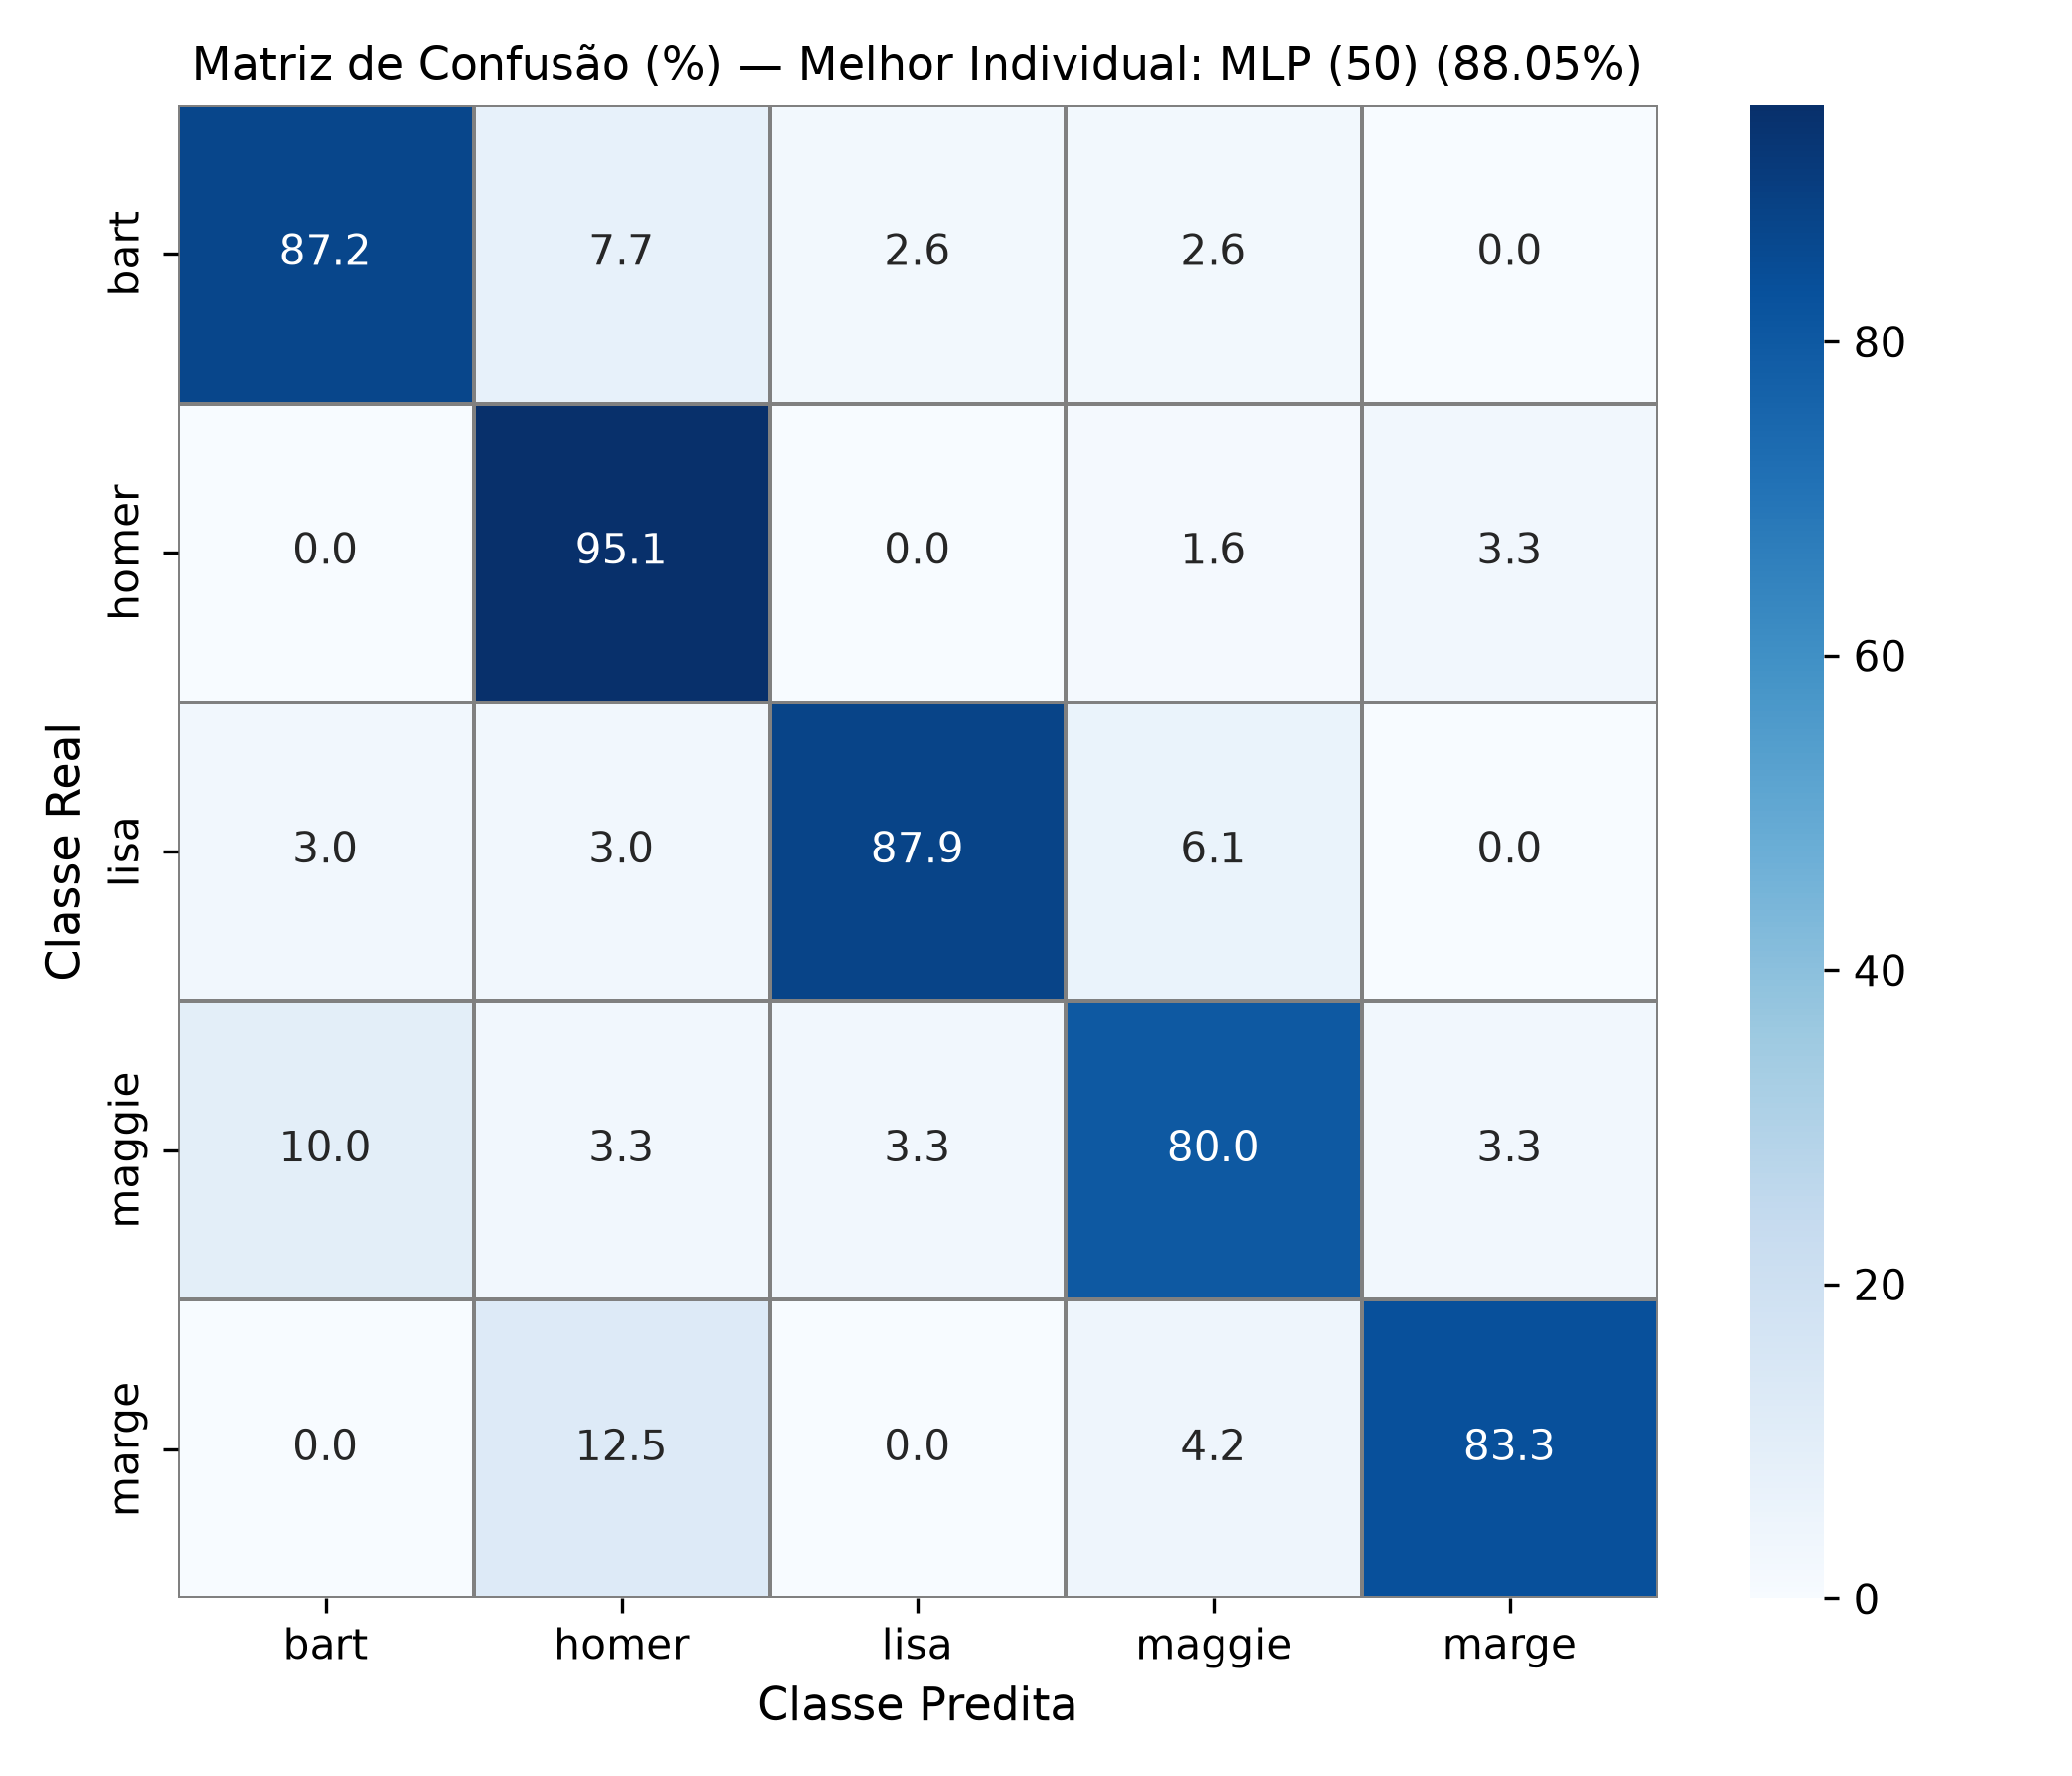
\includegraphics[width=\textwidth]{figs/fig3_matriz_melhor_individual.png}
\end{minipage}
\hfill
\begin{minipage}{0.49\textwidth}
  \centering
  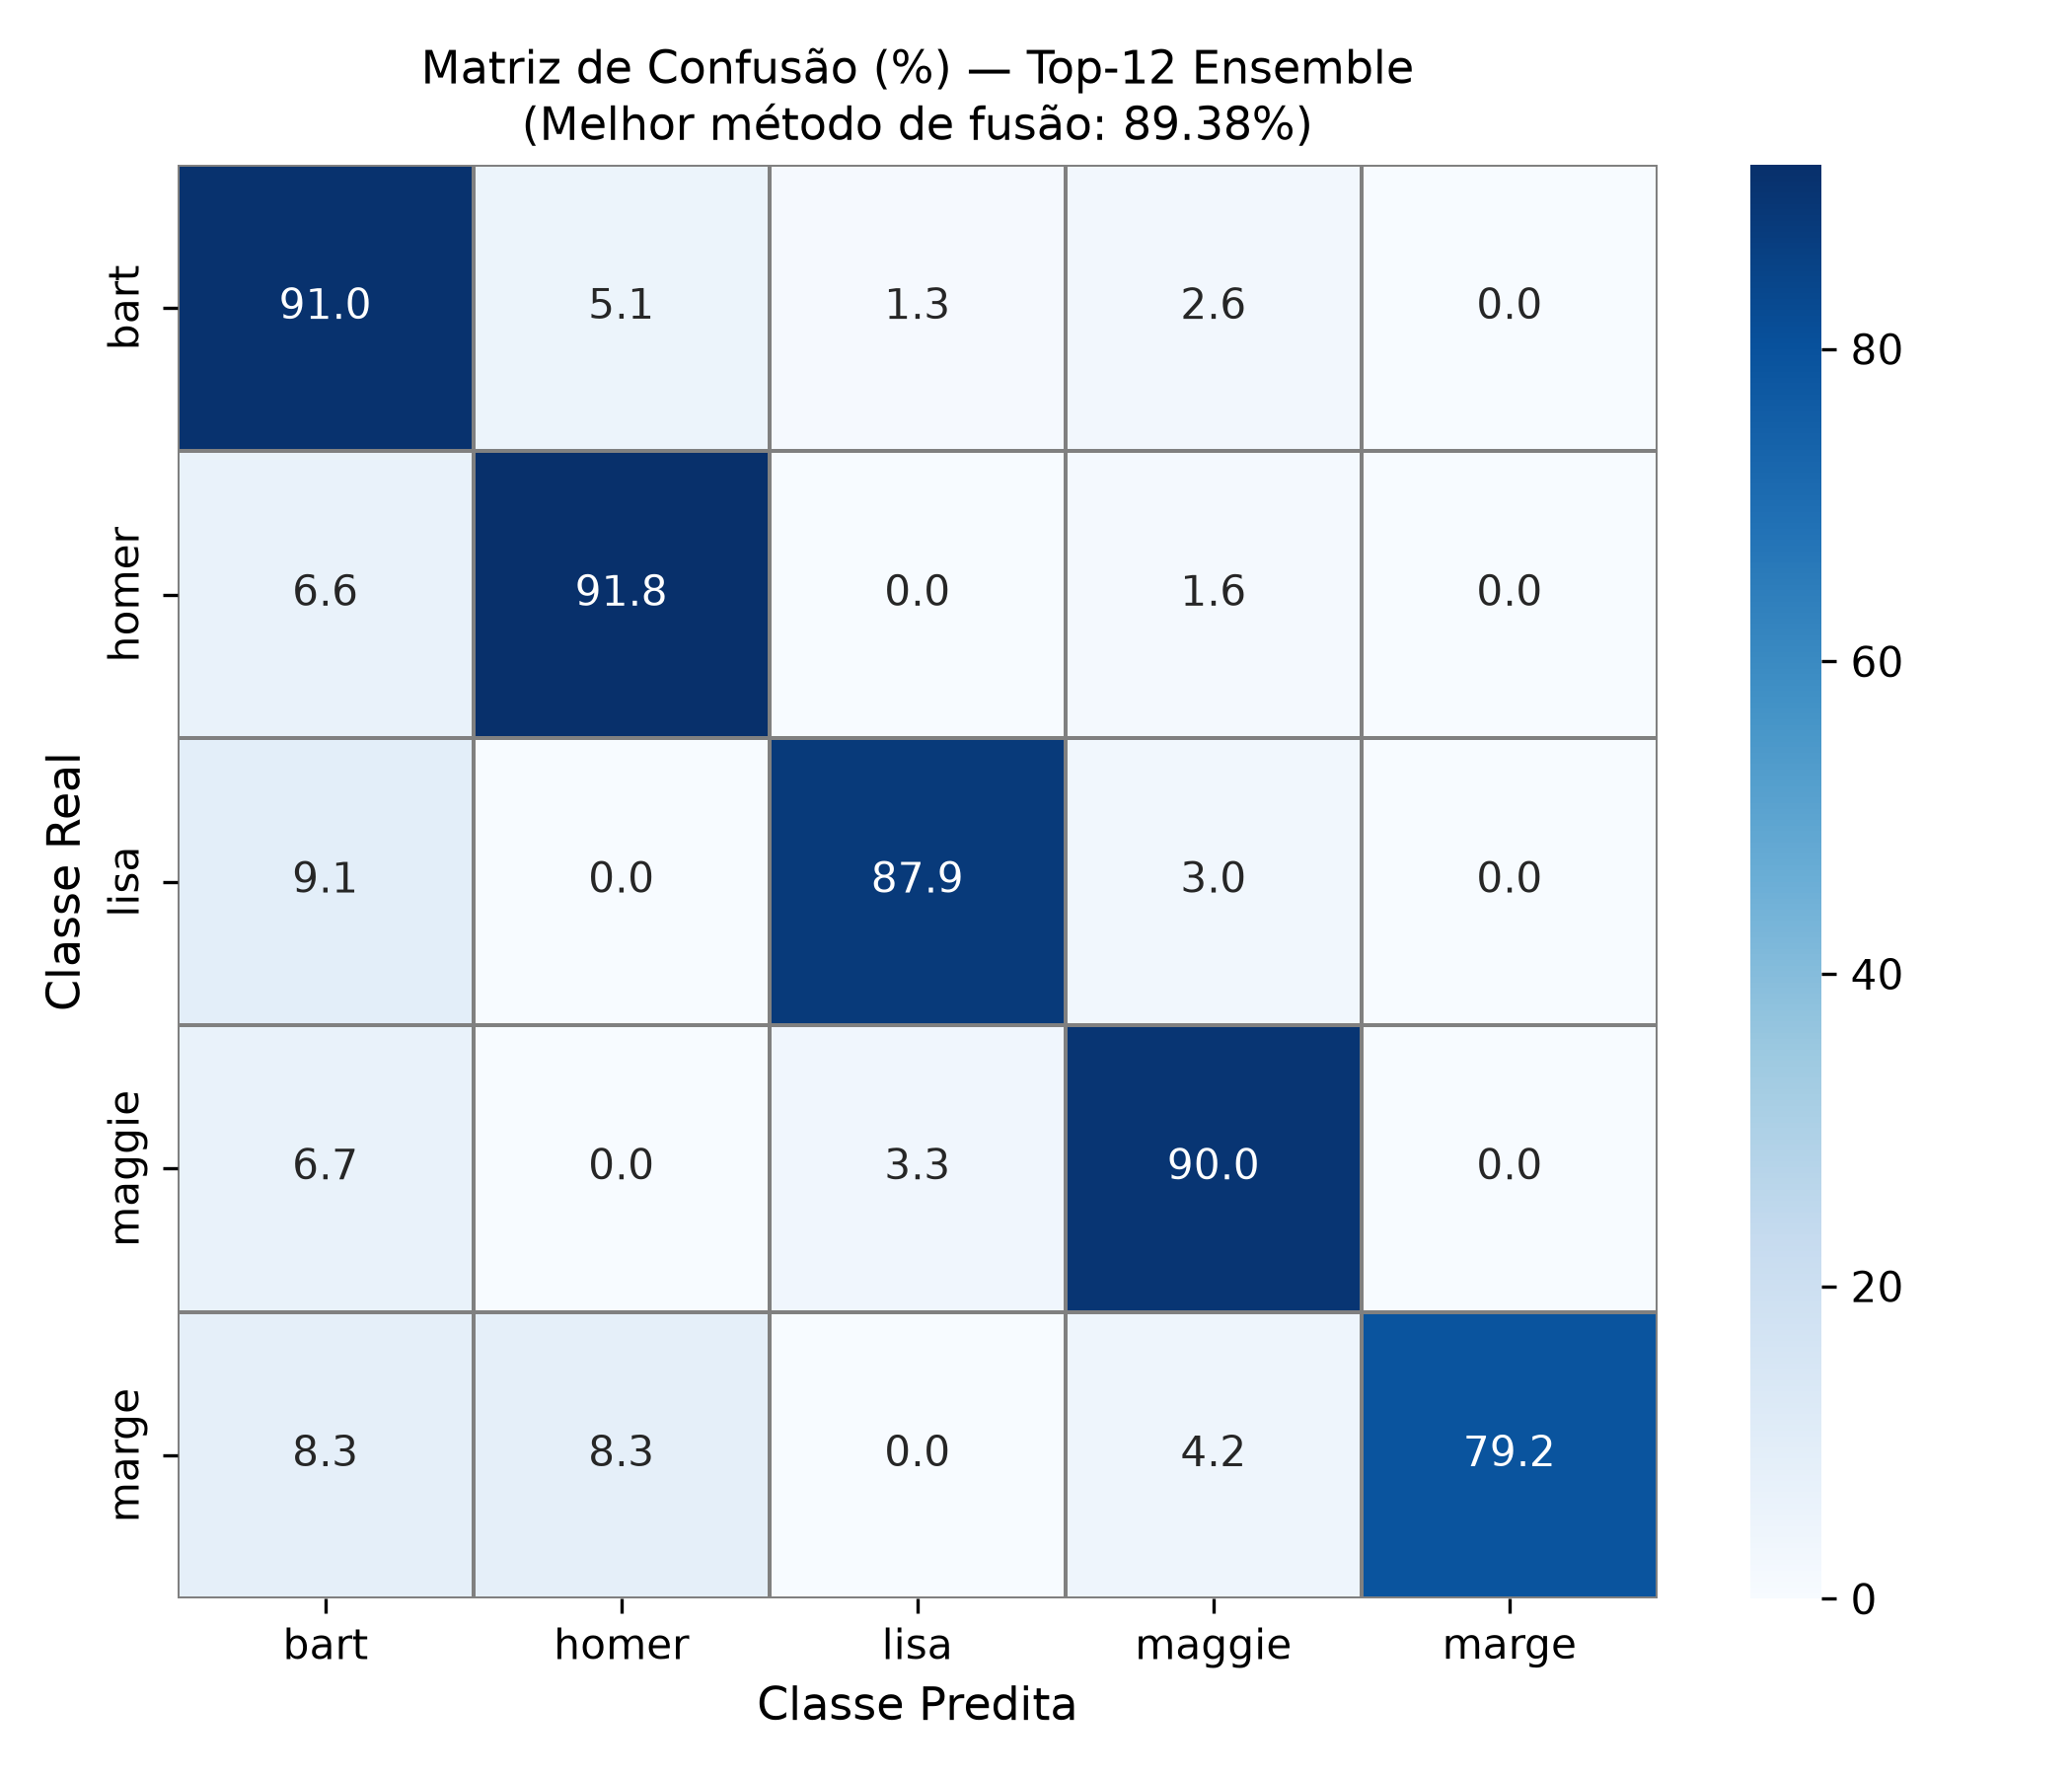
\includegraphics[width=\textwidth]{figs/fig9_matriz_melhor_fusao.png}
\end{minipage}
\caption{Matrizes de confusão (\%) na validação cruzada: melhor individual,
MLP (50) (esquerda), e melhor fusão, Top-12 (direita).}
\label{fig:cm-cv}
\end{figure}

\subsection{Avaliação no Conjunto de Validação (Protocolo B: \textit{holdout})}

Para checar se o sistema generaliza, treinamos todos os modelos no conjunto de
treino completo e os avaliamos no \textit{holdout}, com 95 imagens que não
apareceram no treino. Os resultados estão nas Tabelas~\ref{tab:ind-val}
e~\ref{tab:fusao-val}.

\begin{table}[H]
\centering
\caption{Cinco melhores classificadores individuais no conjunto de validação
(\textit{holdout}).}
\label{tab:ind-val}
\begin{tabular}{lcc}
\toprule
Classificador & Acurácia (\%) & F1-macro (\%) \\
\midrule
\textbf{MLP (50,25)}   & \textbf{84,21} & \textbf{84,56} \\
MLP (100)              & 82,11 & 82,24 \\
MLP (50)               & 81,05 & 79,27 \\
SVM-Linear             & 78,95 & 78,06 \\
SVM-RBF (C=10,0)       & 76,84 & 77,19 \\
\bottomrule
\end{tabular}
\end{table}

\begin{table}[H]
\centering
\caption{Métodos de fusão no conjunto de validação (\textit{holdout}).}
\label{tab:fusao-val}
\begin{tabular}{lcc}
\toprule
Método & Acurácia (\%) & F1-macro (\%) \\
\midrule
Hard Voting (20 clf)          & 77,89 & 77,62 \\
Soft Voting (20 clf)          & 80,00 & 80,35 \\
Weighted Soft Voting (20 clf) & 80,00 & 80,80 \\
Top-5 Ensemble (Soft)         & 80,00 & 79,93 \\
\textbf{Stacking (LR meta-learner)} & \textbf{81,05} & \textbf{80,56} \\
\bottomrule
\end{tabular}
\end{table}

No \textit{holdout}, o melhor modelo isolado foi a MLP (50,25), com 84,21\% de
acurácia; a melhor fusão foi o Stacking, com 81,05\%. Houve uma queda em relação
à validação cruzada, de cerca de 88--89\% para 81--84\%, o que era esperado: o
\textit{holdout} é um conjunto pequeno e totalmente separado do treino (95
imagens), então basta um punhado de casos difíceis para mexer bastante na
estimativa. Aqui vale destacar um ponto: dessa vez a fusão não passou o melhor
individual. A MLP (50,25) generalizou muito bem, ao passo que os métodos de
fusão, por incluírem também os modelos medianos e fracos, acabaram tomando
decisões mais conservadoras. Ainda assim a fusão se segurou perto do topo, com
Stacking e \textit{Soft Voting} acima de 80\%. É esse o seu papel: reduzir a
variância e o risco de apostar tudo num único modelo. Na validação cruzada ela
foi a melhor estratégia; no \textit{holdout} continuou competitiva, sem
despencar. Esse comportamento nos dois protocolos diz bastante sobre a
estabilidade dos classificadores.

\begin{figure}[H]
\centering
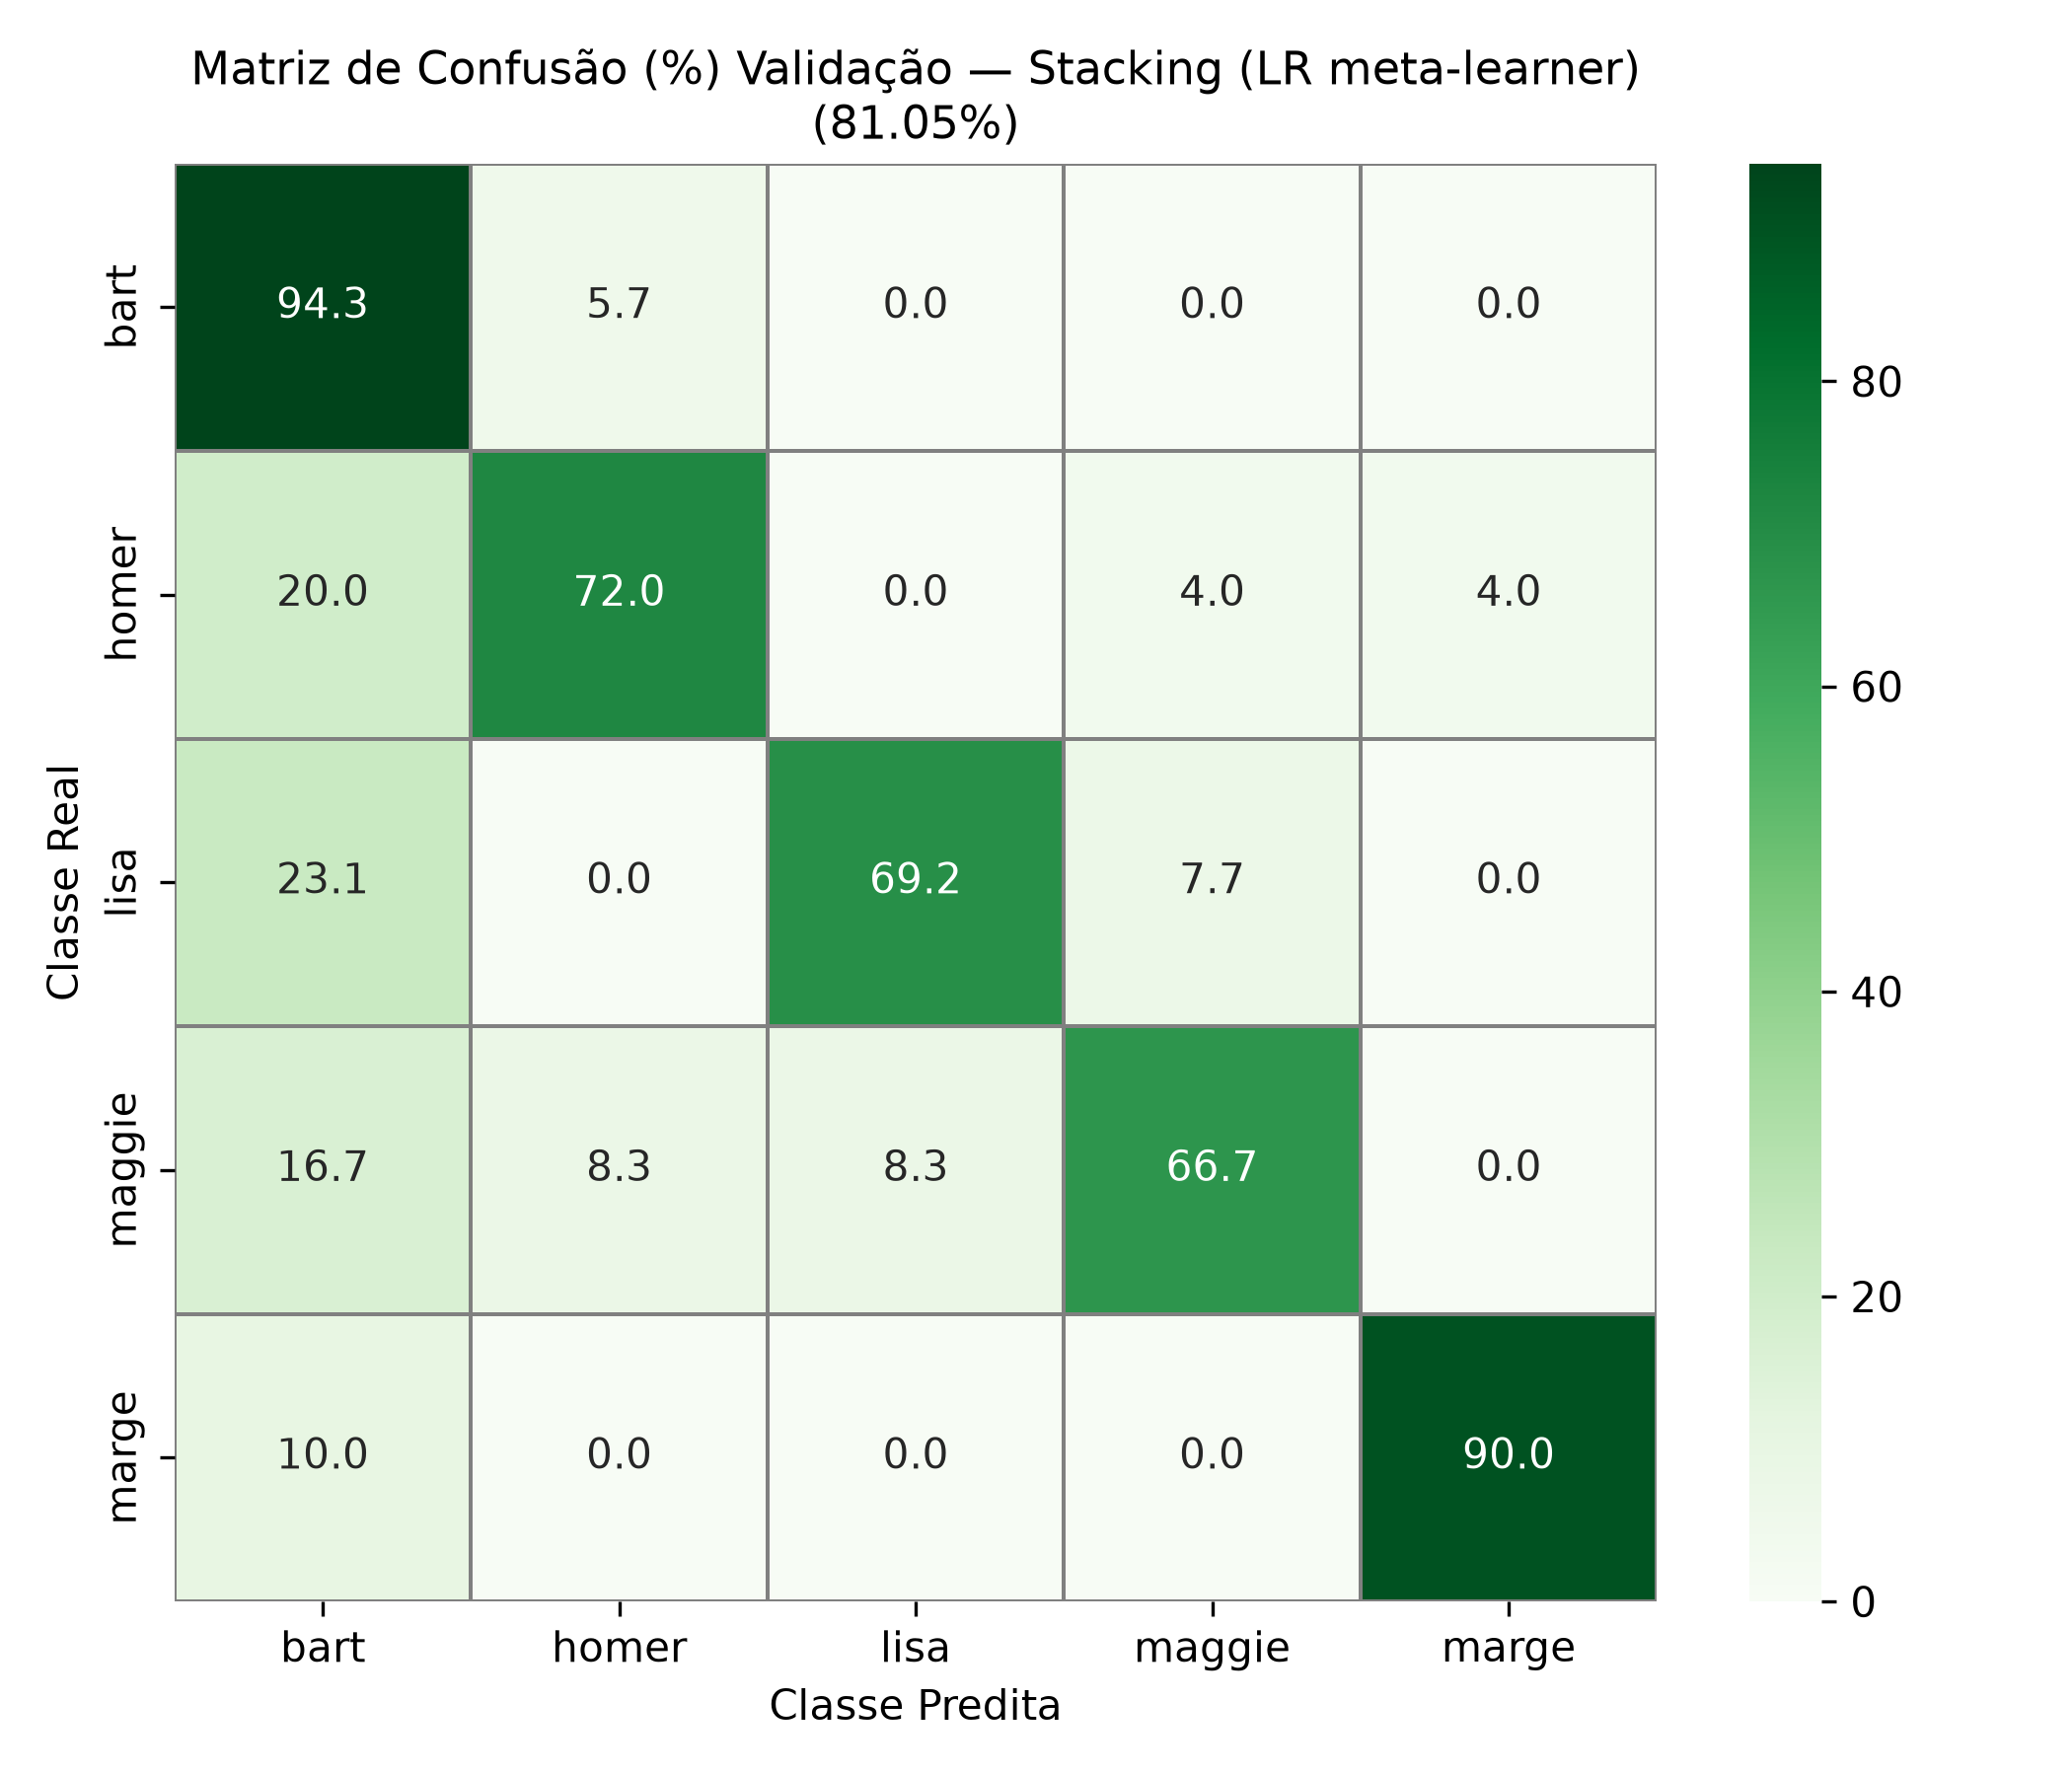
\includegraphics[width=0.50\textwidth]{figs/fig9b_matriz_melhor_fusao_valid.png}
\caption{Matriz de confusão (\%): melhor fusão no conjunto de validação
(\textit{holdout}), Stacking.}
\label{fig:cm-fusao-val}
\end{figure}

\subsection{Pontos Fortes e Fracos do Sistema}

\textbf{Pontos fortes.} As \textit{deep features} do ViT-large puxam a acurácia
para cima mesmo com poucos exemplos por classe, e a fusão seletiva (Top-K e
Stacking) supera o melhor classificador individual de forma consistente. O
F1-macro alto mostra que o sistema vai bem inclusive nas classes minoritárias.

\textbf{Pontos fracos.} O desbalanceamento da base pesa contra Maggie e Marge, de
onde vem a maior parte dos erros. As Árvores de Decisão isoladas rendem pouco e,
quando entram na fusão ingênua, ainda arrastam o \textit{Hard/Soft Voting} para
baixo. Por fim, extrair as \textit{deep features} e rodar o \textit{Stacking} sai
caro em CPU.

% ============================================================
\section{Conclusão}
% ============================================================

Este trabalho montou um sistema para classificar personagens de
\textit{The Simpsons} a partir de \textit{deep features} do ViT-large e de um
\textit{pool} de 20 classificadores combinados por fusão estática. A melhor
configuração foi o \textit{Top-12 Ensemble}, com 89,38\% de acurácia na validação
cruzada de 10 \textit{folds}, 1,33 ponto percentual à frente do melhor modelo
isolado, e os números se mantiveram coerentes no \textit{holdout}. O que os
resultados deixam claro é que fundir de forma \textit{seletiva} rende mais do que
juntar todos os modelos sem critério, e que o grosso dos erros vem do
desbalanceamento entre as classes. Como continuação, dois caminhos parecem
promissores: testar outros descritores, como \textit{deep features} de redes
convolucionais (ResNet ou EfficientNet), e aplicar técnicas de balanceamento para
diminuir as confusões nas personagens com menos exemplos.

\begin{thebibliography}{9}

\bibitem{vit} Dosovitskiy, A. et al. (2021). An Image is Worth 16x16 Words:
Transformers for Image Recognition at Scale. \textit{ICLR}.

\bibitem{sklearn} Pedregosa, F. et al. (2011). Scikit-learn: Machine Learning in
Python. \textit{Journal of Machine Learning Research}, 12, 2825--2830.

\bibitem{ensemble} Kuncheva, L. I. (2014). \textit{Combining Pattern Classifiers:
Methods and Algorithms}. 2nd ed. Wiley.

\bibitem{stacking} Wolpert, D. H. (1992). Stacked Generalization.
\textit{Neural Networks}, 5(2), 241--259.

\end{thebibliography}

\end{document}
